\documentclass[a4paper,11pt]{article}
%\usepackage{amsfonts}
%\usepackage{amssymb}
%\usepackage{amsmath}
%\usepackage{euscript}
%\usepackage{boxedminipage}
\usepackage{lscape}
%\usepackage{minitoc}
%\usepackage{verbatim}
\usepackage{graphicx}
%\usepackage{algpseudocode}
%\usepackage{url,natbib}

\newenvironment{mylisting}
{\begin{list}{}{\setlength{\leftmargin}{1em}}\item\small\bfseries}
{\end{list}}

\vfuzz2pt % Don't report over-full v-boxes if over-edge is small
\hfuzz2pt % Don't report over-full h-boxes if over-edge is small

\setlength{\oddsidemargin}{0cm}
\setlength{\evensidemargin}{0cm}
\setlength{\textwidth}{16cm}
\setlength{\textheight}{24cm}
\setlength{\topmargin}{-1cm}

\begin{document}
\thispagestyle{empty}

% Common EURACE Title Page EURACE and FW6 logos
\vspace{\baselineskip}

\includegraphics[width=45mm]{EURACE-Flag.eps} \hfill

\includegraphics[width=45mm]{eu_6.eps}

% Title
\begin{center}
Project no.\\
035086\\
Project acronym\\
{\bf EURACE}\\
Project title\\
{\bf An Agent-Based software platform for European economic policy design with heterogeneous interacting agents: new insights from a bottom up approach to economic modelling and simulation}\\
\end{center}

\vspace*{\baselineskip}\noindent
Instrument: STREP\\[\baselineskip]
Thematic Priority: IST FET PROACTIVE INITIATIVE ``SIMULATING EMERGENT PROPERTIES IN COMPLEX SYSTEMS\\

% Deliverable information: title & number
\vspace*{2\baselineskip}
\begin{center}
{\bf
%Deliverable reference number and title\\
D5.3: Software module for the agent based models of goods,\\
labour and credit
markets\\ }
Due date of deliverable:\\
31/08/2008\\
Actual submission date:\\
\end{center}


% Project Info
\vspace*{\baselineskip}\noindent
{Start date of project: September 1$^{st}$} 2006 \hfill {Duration: 36 months}\\

%Deliverable Info - partner
\vspace{2\baselineskip}\noindent
Organisation name of lead contractor for this deliverable\\
{\bf University of Sheffield - USFD}
\begin{flushright} 
Revision 1
\end{flushright}

\vspace{\baselineskip}
\begin{table}[hb]
\begin{tabular}{||c|l|l||} \hline\hline
\multicolumn{3}{||l||}{\small Project co-funded by the European Commission within the Sixth Framework Programme (2002-2006)}\\ \hline
\multicolumn{3}{||l||}{\bf Dissemination Level}\\ \hline
\bf PU &\small Public\hfill~& \bf X \\ \hline
\bf PP &\small Restricted to other programme participants (including the Commission Services)& \\ \hline 
\bf RE &\small Restricted to a group specified by the consortium (including the Commission Services)&  \\ \hline
\bf CO &\small Confidential, only for members of the consortium (including the Commission Services)&  \\ \hline \hline
\end{tabular}
\end{table}
\pagebreak
% End of EURACE Title Page

\pagenumbering{roman}
% Table of Contents
\tableofcontents
\pagebreak

% Abstract/SUmmary
\begin{abstract}\noindent
This report presents the deliverable D5.3 accounting for the software
descriptions of the models for the markets - goods and labour and credit markets.
This deliverable acts as part of the work package 5 which comprises of agent
based computational models of goods, labour and credit markets required for the
project EURACE. Also included are sections on general model implementation, as a
lead up to the economic models, and model testing strategies, to make sure the
models are valid.
\end{abstract}
\pagebreak
\pagenumbering{arabic}

% Start of document
In this deliverable we present the internal logical consistency of the fully integrated EURACE model.
Since the focus of WP8 is on the development, integration and validation of the EURACE model, we found it appropriate to restrict D8.5 to these topics. This deliverable therefore does not contain any scenarios or policy experiments, which are collected in WP9.

Chapter 1 describes the construction of a system of national accounts for EURACE, with all the interlinkages between the balance sheets of the agents. We provide a set of accounting rules that should be satisfied for the model to be stock-flow consistent. We have verified that all these rules a true for the fully integrated model, thereby validating the internal logical consistency of all monetary and physical flows.

Chapter 2 on robustness checks shows that the model is robust against changes in critical model parameters and to scaling of the population size. We also show the effects of synchronous versus asynchronous timing of the agents.

Finally, in Chapter 3 we show benchmark results for the Integrated Model that provide the background for the more elaborate policy experiments presented in D9.1-D9.3. 
\section{General Model Implementation}

% Problem, context, solution

Models are constructed from agents that have functions. These functions must be
executed in a correct order for the model to run correctly. Formerly this order
was defined in the model definition XMML by dependencies between functions. These
dependencies could be either internal, within individual agents, or
communication, dependent on messages from other agents. This was enough
information to be able to order functions and plan communication synchronisation
points to work in parallel.

The economic models eventually started to run only certain functions at
certain times, for example, weekly or monthly. Because each function
was still being executed this required a condition at the start of every
function and soon became a hindrance. Even though a series of functions used
the same time series they all had to include the same condition. This was also
true of other conditions, for example only households that were unemployed need
execute functions involved with the labour market.

This was solved by defining the model in the XMML as a state machine. Where
states are defined before and after functions.
Each state can have many incoming functions and many outgoing functions.
Only the unique start state has no incoming functions, and end states have no
outgoing functions. This then allows branches of functions where the condition
for all the functions can be defined at the start of the branch.
An example of this is shown by the similar models in Figures \ref{fig:depends}
and \ref{fig:state}.

\begin{figure}[hb]
\begin{minipage}[b]{0.5\linewidth}
\centering
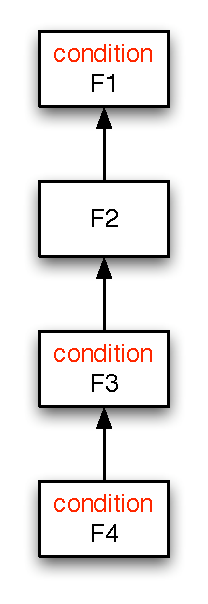
\includegraphics[scale=0.5]{depends_graph.eps}
\caption{Dependency graph model}
\label{fig:depends}
\end{minipage}
\hspace{0.5cm}
\begin{minipage}[b]{0.5\linewidth}
\centering
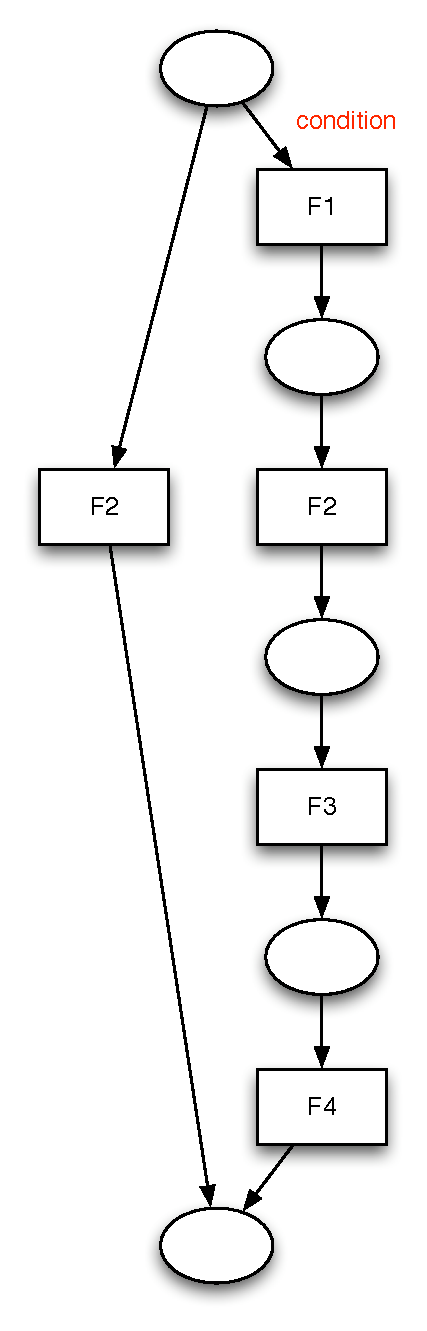
\includegraphics[scale=0.5]{state_graph.eps}
\caption{State graph model}
\label{fig:state}
\end{minipage}
\end{figure}

The model can now be recognised as a state machine but with the restriction
that once a state has been entered by an agent it cannot reenter the same
state. This provides synchronisation of agents in parallel during execution. Also
input to functions are sets of inputs (messages) which can be empty. This is
the level of detail required by FLAME to plan the communication synchronisation
in parallel.

Each function can then be defined by the parameters as shown in Table
\ref{tab:funcparameters}, where $M_{pre}$ is the pre-condition of the memory
and $M_{post}$ is the post-condition of the memory.

\begin{table}[hbp]
\centering
\begin{tabular}{|l|l|l||l||l|l|l|}
\hline
Current State&Input&$M_{pre}$&Function&$M_{post}$&Output&Next State\\
\hline
\end{tabular}
\caption{Function parameters} \label{tab:funcparameters}
\end{table}

In XMML this is currently written as below where $M_{pre}$ is defined as
\textit{condition} and $M_{post}$ is written as source code within a function
with the same name as the function name.

\begin{mylisting}
\begin{verbatim}
<function>
 <name>Function_name</name>
 <description>A description of the function</description>
 <currentState>current_state</currentState>
 <nextState>next_state</nextState>
 <condition>condition</condition>
 <inputs>inputs</inputs>
 <outputs>outputs</outputs>
</function>
\end{verbatim}
\end{mylisting}


\section{Goods and Labour Market Implementation}
The goods and labour market is based on the model presented by the
Bielefeld unit. Detailed description of the model can be found in
D5.1. Here is a brief overview of the implementation of the model.
\subsection{Description}
In order to parse the model and test it for results the labour and
goods market has to be integrated with various models of the credit,
government and financial management markets. Here we concentrate on
the essence of the individual functions involved with the labour and
goods market only. The two main agent involved in this process are
namely - Firms and Households. The state dependency diagram
\ref{fig:statelabour} describes how these functions are interacting
with each other.

\subsubsection{Firm Agent in the Labour and Goods Market}

\begin{landscape}
\begin{table}[!htb]\caption{State Transition Table of the Firm involved in Labour Market.}
\begin{center}
\begin{tabular}{|c|c|c|l|c|c|}
\hline
Function Name & Current State & Next State & Condition & Inputs & Outputs \\
\hline {\parbox[l]{5cm}{Firm \_calculate \_specific \_skills \_and
\_wage \_offer}}& {\parbox[l]{4cm}{Start \_Firm \_Labour \_Role}}&
{\parbox[l]{3cm}{011}}& & & \\
\hline

{\parbox[l]{5cm}{Firm \_send \_vacancies}}& {\parbox[l]{3cm}{011}}&
{\parbox[l]{3cm}{0}}& {\parbox[l]{4cm}{a.no\_employees LT
a.employees\_needed}}& & {\parbox[l]{3cm}{vacancies}}\\
\hline

{\parbox[l]{5cm}{Firm \_send \_redundancies}}&
{\parbox[l]{3cm}{011}}& {\parbox[l]{3cm}{03c}}&
{\parbox[l]{4cm}{a.no\_employees GT a.employees\_needed}} &
 &{\parbox[l]{3cm}{firing}}
\\
\hline

{\parbox[l]{5cm}{Firm \_idle}}& {\parbox[l]{3cm}{011}}&
{\parbox[l]{3cm}{03c}}&{\parbox[l]{4cm}{a.no\_employees EQ
a.employees\_needed}}
 & &
\\
\hline

{\parbox[l]{5cm}{Firm \_read \_job \_applications \_send \_job
\_offer \_or \_rejection}}& {\parbox[l]{3cm}{03}}&
{\parbox[l]{3cm}{04}}& &{\parbox[l]{3cm}{job \_application}}&
{\parbox[l]{3cm}{job\_offer, application\_rejection}}
\\
\hline


{\parbox[l]{5cm}{Firm \_read \_job \_responses}}&
{\parbox[l]{3cm}{04}}& {\parbox[l]{3cm}{05a}}& &
{\parbox[l]{3cm}{job\_acceptance}}&
\\



\hline {\parbox[l]{5cm}{Firm \_read \_job \_quitting}}&
{\parbox[l]{3cm}{05a}}& {\parbox[l]{3cm}{05b}}&&
{\parbox[l]{3cm}{quitting}}
 &
\\
\hline {\parbox[l]{5cm}{Firm \_read \_job \_quitting}}&
{\parbox[l]{3cm}{00b}}& {\parbox[l]{3cm}{09c}}& &
{\parbox[l]{3cm}{quitting}} &
\\
\hline  {\parbox[l]{5cm}{Firm \_read \_job \_quitting}}&
{\parbox[l]{3cm}{03c}}& {\parbox[l]{3cm}{03d}}& &
{\parbox[l]{3cm}{quitting}} & \\
\hline



{\parbox[l]{5cm}{Firm \_start \_labour \_market}}&
{\parbox[l]{3cm}{03d}}&
{\parbox[l]{3cm}{06}}&{\parbox[l]{4cm}{a.no\_employees LT
a.employees\_needed}}
 & &
\\
\hline {\parbox[l]{5cm}{Firm \_finish \_labour \_market \_first
\_round}}& {\parbox[l]{3cm}{03d}}&
{\parbox[l]{3cm}{09a}}&{\parbox[l]{4cm}{a.no\_employees LT
a.employees\_needed}} & &
\\
\hline {\parbox[l]{5cm}{Firm \_finish \_labour \_market \_first
\_round}}& {\parbox[l]{3cm}{05b}}&
{\parbox[l]{3cm}{09a}}&{\parbox[l]{4cm}{a.no\_employees EQ
a.employees\_needed}}
 & &
\\

\hline {\parbox[l]{5cm}{Firm \_update \_wage \_offer}}&
{\parbox[l]{3cm}{05b}}&
{\parbox[l]{3cm}{06}}&{\parbox[l]{4cm}{a.no\_employees LT
a.employees\_needed}}
 & &
\\

\hline {\parbox[l]{5cm}{Firm \_send \_vacancies \_2}}&
{\parbox[l]{3cm}{06}}& {\parbox[l]{3cm}{07}}&
 & & {\parbox[l]{3cm}{vacancies2}}
 \\

\hline {\parbox[l]{5cm}{Firm \_read \_job \_applications \_send
\_job \_offer \_or \_rejection \_2}}& {\parbox[l]{3cm}{07}}&
{\parbox[l]{3cm}{08}}& &{\parbox[l]{3cm}{job\_application2}} &
{\parbox[l]{3cm}{application\_rejection2, job\_offer2}}
\\

\hline {\parbox[l]{5cm}{Firm \_read \_job \_responses \_2}}&
{\parbox[l]{3cm}{08}}& {\parbox[l]{3cm}{09a}}& &
{\parbox[l]{3cm}{job\_acceptance2}} &
\\

\hline {\parbox[l]{5cm}{Firm \_read \_job \_quitting \_2}}&
{\parbox[l]{3cm}{09a}}&
{\parbox[l]{3cm}{09b}}&&{\parbox[l]{3cm}{quitting2}}
 &
\\
\hline {\parbox[l]{5cm}{Firm \_read \_job \_quitting \_2}}&
{\parbox[l]{3cm}{09c}}& {\parbox[l]{4cm}{Start \_Firm \_Seller
\_Role}}&& {\parbox[l]{3cm}{quitting2}}
 &
\\

\hline {\parbox[l]{5cm}{Firm \_update \_wage \_offer \_2}}&
{\parbox[l]{3cm}{09b}}&
{\parbox[l]{3cm}{10}}&{\parbox[l]{4cm}{a.no\_employees LT
a.employees\_needed}}
 & &
\\

\hline {\parbox[l]{5cm}{Firm \_idle}}& {\parbox[l]{3cm}{09b}}&
{\parbox[l]{3cm}{10}}&{\parbox[l]{4cm}{a.no\_employees LT
a.employees\_needed}}
 & &
\\

\hline {\parbox[l]{5cm}{Firm \_compute \_mean \_wage \_specific
\_skills}}& {\parbox[l]{3cm}{10}}& {\parbox[l]{4cm}{End \_Firm
\_Labour \_Role}}&
 & &
\\
\hline


\end{tabular}\end{center}\label{tab:labourfirm}
\end{table}
\end{landscape}

The description of the functions is stated below:
\begin{description}
\item[Firm\_send\_vacancies.] If additional workers are needed the firm sends
vacancies messages
 especially the different wage offers for the different general skill groups.
\item[Firm\_send\_redundancies.] If the firm wants to
decrease the workforce it sends redundancies.
\item[Firm\_idle.] Firm does nothing.
\item[Firm\_read\_job\_applications\_send\_job\_offer\_or\_rejection.] Firm reads the application, ranks the
applicants according to their general and specific skills and sends
as many job offers to the first ranked applicants as the firm has
vacancies to fill. The other applicants are refused.
\item[Firm\_read\_job\_responses.] The firm reads
the responses to their job offers and updates the number of
employees and the number of vacancies.
\item[Firm\_read\_job\_quitting.] The firm reads quitting messages and updates the number
of employees and the number of vacancies.
\item[Firm\_start\_labour\_market.] Dummy function if a firm has to enter the Labor Market
in the second round after receiving quitting.
\item[Firm\_update\_wage\_offer.] The firm increases the wage offer if there are vacancies
 left.
\item[Firm\_send\_vacancies\_2.] If additional workers are needed the firm sends vacancies messages
 especially the different wage offers for the different general skill groups.
\item[Firm\_read\_job\_applications\_send\_job\_offer\_or\_rejection\_2.]
Firm reads the application, ranks the applicants according to their
general and specific skills and sends as many job offers to the
first ranked applicants as the firm has vacancies to fill. The other
applicants are refused.
\item[Firm\_read\_job\_responses\_2.] The firm
reads the responses to their job offers and updates the number of
employees and the number of vacancies.
\item[Firm\_read\_job\_quitting\_2.] The firm reads quitting messages and updates the number
of employees and the number of vacancies.
\item[Firm\_update\_wage\_offer\_2.] The
firm increases the wage offer if there are vacancies left.

\end{description}

\subsubsection{Household Agent in the Labour and Goods Market}

\begin{landscape}
\begin{table}[!htb]\caption{State Transition Table of the Household involved in Labour Market.}
\begin{center}
\begin{tabular}{|c|c|c|l|c|c|}
\hline
Function Name & Current State & Next State & Condition & Inputs & Outputs\\
\hline

{\parbox[l]{5cm}{Household \_read \_firing \_messages}}&
{\parbox[l]{3cm}{Start \_Household \_Labour \_Role}}&
{\parbox[l]{3cm}{01d}}&{\parbox[l]{3cm}{a.employee \_firm \_id NEQ
-1}}
 & {\parbox[l]{3cm}{firing}}&
\\
\hline

{\parbox[l]{5cm}{Household \_idle}}& {\parbox[l]{3cm}{01d}}&
{\parbox[l]{3cm}{01a}}& {\parbox[l]{3cm}{a.employee \_firm \_id EQ
-1}}& &\\
\hline


{\parbox[l]{5cm}{Household \_idle}}& {\parbox[l]{3cm}{Start
\_Household \_Labour \_Role}}& {\parbox[l]{3cm}{01a}}&
{\parbox[l]{3cm}{a.employee \_firm \_id EQ -1}}& & \\
\hline



{\parbox[l]{5cm}{Household \_UNEMPLOYED \_read \_job \_vacancies
\_and \_send \_applications}}& {\parbox[l]{3cm}{01a}}&
{\parbox[l]{3cm}{01}}& & {\parbox[l]{3cm}{vacancies}}
 &{\parbox[l]{3cm}{job \_application}}
\\
\hline

{\parbox[l]{5cm}{Household \_on \_the \_job \_search \_decision}}&
{\parbox[l]{3cm}{01d}}&
{\parbox[l]{3cm}{01b}}&{\parbox[l]{3cm}{a.employee \_firm \_id NEQ
-1}}
 & &
\\
\hline

{\parbox[l]{5cm}{Household \_OTJS \_read \_job \_vacancies \_and
\_send \_applications}}& {\parbox[l]{3cm}{01b}}&
{\parbox[l]{3cm}{01}}&{\parbox[l]{3cm}{a.on\_the\_job\_search EQ
1}}&{\parbox[l]{3cm}{vacancies}}&
{\parbox[l]{3cm}{job\_application}}
\\
\hline


{\parbox[l]{5cm}{Household \_idle}}& {\parbox[l]{3cm}{01b}}&
{\parbox[l]{3cm}{06}}& {\parbox[l]{3cm}{a.on\_the\_job\_search NEQ
1}}&&
\\



\hline {\parbox[l]{5cm}{Household \_read \_job \_offers \_send
\_response}}& {\parbox[l]{3cm}{01}}& {\parbox[l]{3cm}{02}}&&
{\parbox[l]{3cm}{job\_offer}}
 & {\parbox[l]{3cm}{quitting, job\_acceptance}}
\\
\hline {\parbox[l]{5cm}{Household \_finish \_labour \_market}}&
{\parbox[l]{3cm}{02}}& {\parbox[l]{3cm}{06}}&
{\parbox[l]{3cm}{(a.employee\_firm\_id NEQ -1) AND
(a.on\_the\_job\_search NEQ 1)}}&  &
\\
\hline {\parbox[l]{5cm}{Household \_read \_application \_rejection
\_update \_wage \_reservation}}& {\parbox[l]{3cm}{02}}&
{\parbox[l]{3cm}{03}}& {\parbox[l]{3cm}{a.employee\_firm\_id EQ
-1}}& {\parbox[l]{3cm}{application \_rejection}} &
\\
\hline



{\parbox[l]{5cm}{Household \_OTJS \_read \_job \_vacancies \_and
\_send \_applications \_2}}& {\parbox[l]{3cm}{02}}&
{\parbox[l]{3cm}{04}}&{\parbox[l]{3cm}{a.on\_the\_job\_search EQ 1}}
 & {\parbox[l]{3cm}{vacancies2}}&{\parbox[l]{3cm}{job\_application2}}
\\

\hline

{\parbox[l]{5cm}{Household \_UNEMPLOYED \_read \_job \_vacancies
\_and \_send \_applications \_2}}& {\parbox[l]{3cm}{03}}&
{\parbox[l]{3cm}{04}}& & {\parbox[l]{3cm}{vacancies2}}&
{\parbox[l]{3cm}{job\_application2}}
\\
\hline {\parbox[l]{5cm}{Household \_read \_job \_offers \_send
\_response \_2}}& {\parbox[l]{3cm}{04}}& {\parbox[l]{3cm}{05}}&
 &{\parbox[l]{3cm}{job\_offer2}} &{\parbox[l]{3cm}{job\_acceptance2, quitting2}}
\\

\hline {\parbox[l]{5cm}{Household \_read \_application \_rejection
\_update \_wage \_reservation \_2}}& {\parbox[l]{3cm}{05}}&
{\parbox[l]{3cm}{06}}&{\parbox[l]{3cm}{a.employee\_firm\_id EQ -1}}
 & {\parbox[l]{3cm}{application \_rejection2}}&
\\

\hline {\parbox[l]{5cm}{Household \_idle}}& {\parbox[l]{3cm}{05}}&
{\parbox[l]{3cm}{06}}&{\parbox[l]{3cm}{a.employee\_firm\_id NEQ -1}}
 & &
 \\
\hline



\end{tabular}\end{center}\label{tab:labourhh}
\end{table}
\end{landscape}

\begin{description}
\item[Household\_read\_firing\_messages.] The household checks whether is is fired or
 not.
\item[Household\_idle.] Household does nothing.
\item[Household\_UNEMPLOYED\_read\_job\_vacancies\_and\_send\_applications.] Household reads vacancies messages and sends applications.
\item[Household\_on\_the\_job\_search\_decision.] Household decides whether to search on the job or not.
\item[Household\_OTJS\_read\_job\_vacancies\_and\_send\_applications.] Household
searches on the job. Reads vacancies messages and sends
applications.
\item[Household\_read\_job\_offers\_send\_response.] Household reads the job offers and ranks them
according to the wage offer.
\item[Household\_read\_application\_rejection\_update\_wage\_reservation\_2.] Household reads the application rejections and decreases the
reservation wage.
\end{description}




\subsection{Messages being used}



\begin{table}[!htb]\caption{Messages involved in the labour and goods market implementation.}
\begin{center}
\begin{tabular}{|c|l|l|}
\hline
Name & Variables being sent & Description \\
\hline

vacancies & {\parbox[l]{5cm}{firm\_id, region\_id, firm\_vacancies,
skill\_group, firm\_wage\_offer}}& {\parbox[l]{5cm}{Send by firms.
Includes the id, the region id the number of vacancies and the
wage offer for the according general skill level.}} \\

\hline

vacancies2 & {\parbox[l]{5cm}{firm\_id, region\_id, firm\_vacancies,
skill\_group, firm\_wage\_offer}}& {\parbox[l]{5cm}{Send by firms.
Includes the id, the region id the number of vacancies and the
wage offer for the according general skill level.}} \\
\hline

firing & {\parbox[l]{5cm}{firm\_id, worker\_id}}
& {\parbox[l]{5cm}{Send by firms. Includes the id and the id of the dismissed employee.}}  \\

\hline

job\_application & {\parbox[l]{5cm}{worker\_id, firm\_id,
region\_id, general\_skill, specific\_skill}} &
{\parbox[l]{5cm}{Send by households to apply for a job. Includes the
id, firm id, region id the general
as well as the specific skills.}}   \\
\hline


job\_application2 & {\parbox[l]{5cm}{worker\_id, firm\_id,
region\_id, general\_skill, specific\_skill}} &
{\parbox[l]{5cm}{Send by households to apply for a job. Includes the
id, firm id, region id the general
as well as the specific skills.}}   \\
\hline


job\_offer & {\parbox[l]{5cm}{ firm\_id,worker\_id, region\_id,
wage\_offer}} & {\parbox[l]{5cm}{Send by firms to make a job offer
for a household. Includes the id, worker id and the
corresponding wage offer.}}   \\

\hline


job\_offer2 & {\parbox[l]{5cm}{ firm\_id,worker\_id, region\_id,
wage\_offer}} & {\parbox[l]{5cm}{Send by firms to make a job offer
for a household. Includes the id, worker id and the
corresponding wage offer.}}   \\
\hline


job\_acceptance & {\parbox[l]{5cm}{worker\_id, firm\_id, region\_id,
general\_skill, specific\_skill}} & {\parbox[l]{5cm}{Send by
households to accept the job offer. Includes the id, firm id, region
id, the general
as well as the specific skills.}}   \\
\hline



job\_acceptance2 & {\parbox[l]{5cm}{worker\_id, firm\_id,
region\_id, general\_skill, specific\_skill}} &
{\parbox[l]{5cm}{Send by households to accept the job offer.
Includes the id, firm id, region id, the general
as well as the specific skills.}}   \\
\hline

application\_rejection & {\parbox[l]{5cm}{firm\_id, worker\_id}} &
{\parbox[l]{5cm}{Send by firms. Includes the id and the id of the refused applicant.}}   \\
\hline

application\_rejection2 & {\parbox[l]{5cm}{firm\_id, worker\_id}} &
{\parbox[l]{5cm}{Send by firms. Includes the id and the id of the refused applicant.}}   \\
\hline

quitting & {\parbox[l]{5cm}{worker\_id, firm\_id}} &
{\parbox[l]{5cm}{Send by households to quit the current job. Includes the id, firm id.}}   \\
\hline

quitting2 & {\parbox[l]{5cm}{worker\_id, firm\_id}} &
{\parbox[l]{5cm}{Send by households to quit the current job. Includes the id, firm id.}}   \\
\hline

\end{tabular}\end{center}\label{tab:labourmarketmsg}
\end{table}


 \begin{figure}[!htb]
 \begin{center}
 \includegraphics*[scale=2.0]{stategraph-labour.ps}
 \caption{State Dependency Diagram of the Labour Market Model.} \label{fig:statelabour}
 \end{center}
 \end{figure}

\section{Credit Market Implementation}

This model was adapted from the proposed model of the credit market
by the Ancona Unit \cite{?}. Here we present a description of how
the model was implemented.

\subsection{Description}
The credit market involves the interaction of the credit function
with the financial management functions of the Firm and Bank agent.
The state dependency diagram \ref{fig:statecredit} shows the flow of
activity in the model.

% \subsection{Agents}
% The agents involved in the implementation are listed below:
% \begin{itemize}
% \item Bank Agent - reads loans requests and approves loans.
% \item Firm Agent - requests for loans if needed.
% \item Dummy Agent - to handle message of orders and household
% functions.
% \end{itemize}
%
% \subsection{State dependency diagram}
%
% \begin{figure}[!htb]
% \begin{center}
%  \includegraphics*[scale=2.0]{stategraph.ps}
% \caption{State Dependency Diagram.} \label{fig:statecredit}
% \end{center}
% \end{figure}
%
% The state dependency diagram \ref{fig:statecredit} shows the flow of
% activity in the model. The details of the functions of the agents
% can be found in the report presented by the Ancona Unit \cite{?}.
%
% The xmml file for the credit market can be found in the Chapter
% \ref{appendix}.
%
% \section{Results}
% Graphs


 \begin{figure}[!htb]
 \begin{center}
  \includegraphics*[scale=2.0]{stategraph.ps}
 \caption{State Dependency Diagram.} \label{fig:statecredit}
 \end{center}
 \end{figure}


\subsubsection{Firm Agent in the Credit Market}


\begin{landscape}
\begin{table}[!htb]\caption{Functions being performed by the Firm involved in Credit Market.}
\begin{center}
\begin{tabular}{|c|c|c|l|c|c|l|}
\hline
Function Name & State From & State to & Condition on Function & Inputs & Outputs & Description \\
\hline
{\parbox[l]{3cm}{Firm \_ask \_loan}}&
{\parbox[l]{3cm}{Start \_Firm \_Credit \_Role}}&
{\parbox[l]{3cm}{Firm \_Credit \_02}}&
{\parbox[l]{3cm}{a.external \_financial \_needs GT 0.0}}
&
&loan \_request &
\\
\hline

{\parbox[l]{3cm}{Firm \_get \_loan}}& {\parbox[l]{3cm}{Firm \_Credit
\_02}}& {\parbox[l]{3cm}{Firm \_End \_Credit \_Role}}&
&{\parbox[l]{3cm}{loan \_conditions ( a.id EQ m.firm\_id}} &
{\parbox[l]{3cm}{loan \_acceptance}}&\\
\hline


\end{tabular}\end{center}\label{tab:creditbankfn}
\end{table}
\end{landscape}

\subsubsection{Bank Agent in the Credit Market}



\begin{landscape}
\begin{table}[!htb]\caption{Functions being performed by the Bank involved in Credit Market.}
\begin{center}
\begin{tabular}{|c|c|c|l|c|c|l|}
\hline
Function Name & State From & State to & Condition on Function & Inputs & Outputs & Description \\
\hline

{\parbox[l]{3cm}{Bank \_decide \_credit \_conditions}} &
{\parbox[l]{3cm}{Bank \_start \_credit \_market \_role}} & Bank\_02
& & {\parbox[l]{3cm}{loan\_request (a.id EQ m.bank\_id)}} &
{\parbox[l]{3cm}{loan \_conditions}} &\\

\hline

{\parbox[l]{3cm}{Bank \_give \_loan}} & Bank\_02 & Bank\_03 & &
{\parbox[l]{3cm}{loan \_acceptance (a.id EQ m.bank \_id)}} &  &\\

\hline

{\parbox[l]{3cm}{Bank \_receive \_installment}} & Bank\_03 &
Bank\_04 & &
{\parbox[l]{3cm}{installment (a.id EQ m.bank\_id)}} & & \\

&&&&
{\parbox[l]{3cm}{bankruptcy (a.id EQ m.bank\_id)}} &  &\\

\hline


{\parbox[l]{3cm}{Bank \_account \_update \_deposits}} & Bank\_04 &
Bank\_05 & & {\parbox[l]{3cm}{bank\_account \_update (a.id EQ
m.bank\_id)}} &
{\parbox[l]{3cm}{central \_bank \_account \_update}} &\\

\hline


{\parbox[l]{3cm}{Bank \_accounting}} & Bank\_05 &
{\parbox[l]{3cm}{end \_Bank \_cycle}} &
{\parbox[l]{4cm}{monthly (a.day \_of \_month \_to \_act)}}&  &  &\\

\hline


{\parbox[l]{3cm}{Bank\_idle}} & Bank\_05 & {\parbox[l]{3cm}{end
\_Bank \_cycle}} &
{\parbox[l]{4cm}{not (monthly (a.day \_of \_month \_to \_act))}}&  &  &\\
\hline


\end{tabular}\end{center}\label{tab:creditbankfn}
\end{table}
\end{landscape}

\subsection{Messages being Used}



\begin{table}[!htb]\caption{Messages involved in the credit market implementation.}
\begin{center}
\begin{tabular}{|c|l|l|}
\hline
Name & Variables being sent & Description \\
\hline loan\_request & {\parbox[l]{5cm}{firm\_id, bank\_id, equity,
total\_debt, external\_financial\_needs}}& {\parbox[l]{5cm}{Message
added by firm to demand credit with bank\_id,
with financial info of applying firm.}} \\
\hline loan\_conditions & {\parbox[l]{5cm}{firm\_id, bank\_id,
proposed\_interest\_rate, amount\_offered\_credit, value\_at\_risk}}
& {\parbox[l]{5cm}{Message added by bank to offer credit, contains
the interest rate, the amount of
offered credit, and the value\_at\_risk.}}  \\

\hline loan\_acceptance & {\parbox[l]{5cm}{bank\_id,
credit\_amount\_taken, loan\_total\_var}} & {\parbox[l]{5cm}{Message
added by firm to accept a loan with bank\_id, for the amount credit
taken and VAR. The bank
does not need to know the firm\_id.}}   \\
\hline

installment & {\parbox[l]{5cm}{bank\_id, installment\_amount,
interest\_amount, var\_per\_installment}} & {\parbox[l]{5cm}{Message
added by firm pays
installment and interest to the bank.}}    \\

\hline bankruptcy & {\parbox[l]{5cm}{bank\_id, bad\_debt,
credit\_refunded, residual\_var}} &{\parbox[l]{5cm}{Message added by
firm to bank
to signal bankruptcy.}}  \\
\hline BCE\_return &
{\parbox[l]{5cm}{bce\_debt, id}} & {\parbox[l]{5cm}{}}  \\
\hline

\end{tabular}\end{center}\label{tab:creditmarketmsg}
\end{table}

\subsection{Unit testing of the message board API}
As mentioned above the message boards (are accessed by the FLAME framework via a Application Program Interface - the Message Board Library (the libmboard API). This provides the FLAME developer with a uniform interface to the functionality of the libmboard.
\subsection{Testing serial and parallel implementations}
It is important to ensure that application generated by the FLAME framework execute \textsl{correctly} in both their serial and parallel modes. Because of the stocastic nature of the agent-based approach to modelling it is unrealistic to expect complex simulations to following exactly the solution path although general trends should be similar. However for some simple applications we can expect to serial and parallel implementations to produce exactly the results throughout the simulation. Such example applications can be used to verify the correctness of both the serial and parallel implementations.

The \textsl{Circles Model} is one such application. The \textsl{Circles} agent is very simple. It has a position in two-dimensional space and a radius of influence. Each agent will react to its neighbours within its interaction radius repulsively. So given a sufficient simulation time the initial distribution of agents will tend to a field of uniformly spaced agents. Each agent has $x$, $y$, $fx$, $fy$ and $radius$ in its memory and has three states: outputdata, inputdata and move. The agents communicate via a single message board, $location$, which holds the agent $id$ and position. Given the simplicity of the agent it is possible to determine the final result of a number of ideal models.

A set of simple test models and problems have been developed based on the \textsl{Circles} agent. Each test has a \textsl{model.xmml} files and a set of initial data (\textsl{0.xml}).
\begin{description}
	\item [Test 1]: Model: single \textsl{Circles} agent type; Initial population of no agents. Expected result:
	\item [Test 2]: Model: single \textsl{Circles} agent type; Initial population of one agent at (0,0).
\end{description}


%In this report we have described the parallel implementation of the FLAME framework and its assessment together with some benchmarking results using the EURACE Model. We have also demonstrated FLAMEs use in a number of EURACE related simulations in addition to complete EURACE model on populations ranging from a few hundereds of agents, through tens of thousands to, in one case, a million agents.  In some of these simulations the parallel implementation of FLAME has shown reasonable scalability and parallel efficiency but in other the results have been disappointing.

An important goal of the project has been to perform, in parallel, a large simulation using the EURACE Model. The project has achieve this to a degree: the model has been defined, important parameters have been values, a method of generating agent populations implemented and a parallel implementation of the EURACE model can be generated by FLAME. Using these steps serial and parallel simulations of the EURACE Model have been perform. In this process a detail assessment of the FLAME generated code, the serial and parallel implementations and the EURACE Model have been performed. Message counts, function times and sychronisation times are a few of the measures that have been used together with a detail static analysis of the model to identify the performance defficiencies in both the FLAME framework and the EURACE model.

All this analysis has lead to improvements in FLAME and the EURACE Model which in general have improved its computational performance. However the presence of substanial serial components in any model has resulted in very poor parallel scalability. It is well known that parallel speedup is limited by the serial faction of a code - this is Amdah's Law. The analyses performed on the EURACE Model have shown that the singleton agents - in particularly the Clearing House - have a significant impact of the parallel performance of the model.
These types of potential problem were understood - fine grained tasks - at the start of the project and the modeller took steps to avoid them. The Clearing House was thought necessary to the architecture of the EURACE Model and although different strategies were tested to reduce its effect there was little that could be achieved. The Clearing House and any other serial bottleneck will compromise the parallel performance of the application.

Although at the end of EURACE we have not achieved the \textsl{optimum} solution to these problems we have at least advanced the current state of the art in the parallel implementation of agent-based simulations in the context of the FLAME Framework.

%\bibliographystyle{alpha}
\bibliographystyle{plain}
\bibliography{EURACE_refs}
% End of document
\end{document}
